% Green Sand Near-Infrared Reference Library and Detection-Limit Benchmark
% Every number in this file comes from macros.tex and tables/*.tex, generated by
% code/09_preprint_assets.py from the pipeline outputs (paper/stats.json).
\documentclass[10pt,twocolumn,letterpaper]{article}
\usepackage[T1]{fontenc}
\usepackage[utf8]{inputenc}
\usepackage{mathpazo}
\usepackage[letterpaper,top=0.8in,bottom=0.85in,left=0.7in,right=0.7in,columnsep=0.28in]{geometry}
\usepackage{amsmath,amssymb}
\usepackage{graphicx}
\usepackage{booktabs}
\usepackage{array}
\usepackage{xcolor}
\usepackage{pifont}
\usepackage[sort&compress,numbers,square]{natbib}
\usepackage{titlesec}
\usepackage[font=small,labelsep=colon,justification=centering,singlelinecheck=false]{caption}
\usepackage{microtype}
\usepackage{fancyhdr}
\usepackage{dblfloatfix}
\definecolor{linkblue}{HTML}{1C5CAB}
\usepackage[colorlinks=true,linkcolor=linkblue,citecolor=linkblue,urlcolor=linkblue]{hyperref}
\usepackage{orcidlink}

% Generated by code/09_preprint_assets.py from paper/stats.json. Do not edit by hand.
\newcommand{\alphaFourteen}{31}
\newcommand{\alphaNineteen}{124}
\newcommand{\dropMeas}{0.115}
\newcommand{\dropLin}{0.010}
\newcommand{\dropHapke}{0.088}
\newcommand{\dropRatio}{11}
\newcommand{\mmHematiteGrainUm}{8.8}
\newcommand{\mmHematiteToQuartzSizeRatio}{0.22}
\newcommand{\mmQuartzScale}{1.059}
\newcommand{\mmRmseHapke}{0.0112}
\newcommand{\mmRmseLinear}{0.0222}
\newcommand{\mmRthousandMeasured}{0.776}
\newcommand{\mmRthousandHapke}{0.803}
\newcommand{\mmRthousandLinear}{0.881}
\newcommand{\rmseRaw}{187}
\newcommand{\rmseOff}{36.7}
\newcommand{\rmseOffOnly}{106.4}
\newcommand{\labAucSd}{119.4}
\newcommand{\labAucMin}{102}
\newcommand{\labAucMax}{525}
\newcommand{\dSc}{37.7}
\newcommand{\dFe}{2.48}
\newcommand{\dScLo}{33.1}
\newcommand{\dScHi}{48.9}
\newcommand{\dFeLo}{1.30}
\newcommand{\dFeHi}{3.66}
\newcommand{\offThree}{50}
\newcommand{\offSix}{172}
\newcommand{\offNine}{159}
\newcommand{\offTwelve}{278}
\newcommand{\residMaxAbs}{96}
\newcommand{\rFitSc}{0.92}
\newcommand{\rFitFe}{0.92}
\newcommand{\offAbsLo}{0.037}
\newcommand{\offAbsHi}{0.206}
\newcommand{\filmThreeFive}{1.05}
\newcommand{\RnineteenDry}{0.430}
\newcommand{\RnineteenWetTwo}{0.415}
\newcommand{\RnineteenWetFive}{0.393}
\newcommand{\thrSc}{0.23}
\newcommand{\thrFe}{0.07}
\newcommand{\rmsepSc}{0.38}
\newcommand{\rmsepFe}{0.14}
\newcommand{\trendsCal}{5}
\newcommand{\pcScCal}{99.78}
\newcommand{\pcFeCal}{95.61}
\newcommand{\trendsUsgs}{3}
\newcommand{\pcScUsgs}{99.39}
\newcommand{\pcFeUsgs}{90.68}
\newcommand{\trendsLin}{2}
\newcommand{\pcScLin}{96.30}
\newcommand{\pcFeLin}{88.39}
\newcommand{\lodScDryIdeal}{0.3}
\newcommand{\rmsecvScDryIdeal}{0.18}
\newcommand{\rtwoScDryIdeal}{0.972}
\newcommand{\lodScDryLab}{0.5}
\newcommand{\rmsecvScDryLab}{0.27}
\newcommand{\rtwoScDryLab}{0.938}
\newcommand{\lodScDryPlant}{0.75}
\newcommand{\rmsecvScDryPlant}{0.38}
\newcommand{\rtwoScDryPlant}{0.883}
\newcommand{\lodScMoistIdeal}{0.5}
\newcommand{\rmsecvScMoistIdeal}{0.16}
\newcommand{\rtwoScMoistIdeal}{0.976}
\newcommand{\lodScMoistLab}{0.5}
\newcommand{\rmsecvScMoistLab}{0.26}
\newcommand{\rtwoScMoistLab}{0.951}
\newcommand{\lodScMoistPlant}{0.75}
\newcommand{\rmsecvScMoistPlant}{0.34}
\newcommand{\rtwoScMoistPlant}{0.917}
\newcommand{\lodFeDryIdeal}{0.1}
\newcommand{\rmsecvFeDryIdeal}{0.10}
\newcommand{\rtwoFeDryIdeal}{0.953}
\newcommand{\lodFeDryLab}{0.1}
\newcommand{\rmsecvFeDryLab}{0.11}
\newcommand{\rtwoFeDryLab}{0.948}
\newcommand{\lodFeDryPlant}{0.15}
\newcommand{\rmsecvFeDryPlant}{0.12}
\newcommand{\rtwoFeDryPlant}{0.931}
\newcommand{\lodFeMoistIdeal}{0.15}
\newcommand{\rmsecvFeMoistIdeal}{0.09}
\newcommand{\rtwoFeMoistIdeal}{0.954}
\newcommand{\lodFeMoistLab}{0.15}
\newcommand{\rmsecvFeMoistLab}{0.10}
\newcommand{\rtwoFeMoistLab}{0.954}
\newcommand{\lodFeMoistPlant}{0.2}
\newcommand{\rmsecvFeMoistPlant}{0.12}
\newcommand{\rtwoFeMoistPlant}{0.921}
\newcommand{\moistScDef}{0.5}
\newcommand{\moistFeDef}{0.1}
\newcommand{\moistScPf}{0.5}
\newcommand{\moistFePf}{0.15}
\newcommand{\sensScLin}{4}
\newcommand{\sensFeLin}{1}
\newcommand{\sensScCb}{0.3}
\newcommand{\sensFeCb}{0.1}
\newcommand{\sensScSaz}{0.3}
\newcommand{\sensFeSaz}{0.15}
\newcommand{\sensScClay}{0.5}
\newcommand{\sensFeClay}{0.1}
\newcommand{\sensScFwhm}{0.5}
\newcommand{\sensFeFwhm}{0.1}
\newcommand{\sensScUsgs}{0.3}
\newcommand{\sensFeUsgs}{0.15}
\newcommand{\wMix}{0.87516}
\newcommand{\RMix}{0.47784}
\newcommand{\xsSand}{0.23}
\newcommand{\xsClay}{0.59}
\newcommand{\xsSc}{0.11}
\newcommand{\xsFe}{0.07}
\newcommand{\nDry}{4{,}410}
\newcommand{\nMoist}{6{,}930}
\newcommand{\nTotal}{11{,}340}
\newcommand{\nNative}{1{,}351}
\newcommand{\nInst}{195}
\newcommand{\nCal}{600}
\newcommand{\nTestBlank}{200}
\newcommand{\nTestLevel}{100}
\newcommand{\nSets}{12}
\newcommand{\nTestSc}{1{,}600}
\newcommand{\nTestFe}{1{,}400}
\newcommand{\levelsSc}{0.02, 0.05, 0.1, 0.15, 0.2, 0.3, 0.5, 0.75, 1, 1.5, 2, 3, 4, 5}
\newcommand{\levelsFe}{0.01, 0.02, 0.05, 0.1, 0.15, 0.2, 0.3, 0.5, 0.75, 1, 1.5, 2}
\newcommand{\feFullShare}{91.4}
\newcommand{\snrIdeal}{10{,}000}
\newcommand{\snrLab}{2{,}000}
\newcommand{\snrPlant}{500}
\newcommand{\spotId}{GSNIR-v1.0-02462}
\newcommand{\spotR}{0.47784}
\newcommand{\powScThree}{0.74}
\newcommand{\powFeFive}{0.45}
\newcommand{\svmFive}{0.00}
\newcommand{\svmOne}{1.00}
\newcommand{\rfFeTwo}{0.60}

\makeatletter\newcommand{\tabinput}[1]{\@@input #1 }\makeatother
\newcommand{\cmark}{\ding{51}}
\newcommand{\xmark}{\ding{55}}
\newcommand{\um}{\,$\mu$m}

% REVTeX-like look: Roman-numeral small-caps sections, lettered subsections
\renewcommand{\thesection}{\Roman{section}}
\renewcommand{\thesubsection}{\Alph{subsection}}
\titleformat{\section}{\centering\normalfont\small\bfseries}{\thesection.}{0.6em}{\MakeUppercase}
\titlespacing*{\section}{0pt}{2.2ex plus 0.5ex}{1.2ex}
\titleformat{\subsection}{\centering\normalfont\small\bfseries}{\thesubsection.}{0.5em}{}
\titlespacing*{\subsection}{0pt}{1.8ex plus 0.5ex}{1.0ex}
\titleformat{\subsubsection}{\normalfont\small\itshape}{\thesubsubsection.}{0.5em}{}
\renewcommand{\thesubsubsection}{\arabic{subsubsection}}
\renewcommand{\thetable}{\Roman{table}}
\captionsetup[figure]{name=FIG.}
\captionsetup[table]{name=TABLE,position=top}
\setlength{\parindent}{1.2em}
\setlength{\textfloatsep}{10pt plus 2pt minus 2pt}
\setlength{\dbltextfloatsep}{10pt plus 2pt minus 2pt}
\renewcommand{\arraystretch}{1.12}

\pagestyle{fancy}
\fancyhf{}
\fancyhead[R]{\small\thepage}
\renewcommand{\headrulewidth}{0pt}
\fancypagestyle{plain}{\fancyhf{}\renewcommand{\headrulewidth}{0pt}}

\begin{document}

\twocolumn[
\begin{center}
{\large\bfseries Open Near-Infrared Reference Library and Detection-Limit Benchmark\\[2pt] for Seacoal and Red Iron Oxide in Foundry Green Sand\par}
\vspace{10pt}
{\normalsize Maurice Kuubata\,\orcidlink{0009-0003-3178-5971}\par}
\vspace{3pt}
{\small\itshape Independent Researcher, Dubuque, Iowa, USA\par}
\vspace{2pt}
{\small Correspondence: \href{mailto:kuubatamaurice@gmail.com}{kuubatamaurice@gmail.com}\par}
\vspace{10pt}
\begin{minipage}{0.80\textwidth}
\small
Green sand additive control still relies on slow offline tests such as loss on ignition, so out-of-specification sand can reach the molding line before results return. Near-infrared (NIR) spectroscopy can read sand in seconds, but no open reference exists that tells a foundry, a sensor maker, or a researcher which additive levels an NIR method can actually detect. We present an open, versioned library of \nTotal{} computed NIR reflectance spectra of foundry green sand (\nDry{} dry mixtures spanning 3--12\% bentonite, 0--5\% seacoal and 0--2\% red iron oxide, plus \nMoist{} mixtures at 2--5\% moisture), together with a detection-limit benchmark and a tested Python package. Spectra are computed from U.S. Geological Survey Spectral Library Version 7 reference spectra by Hapke single-scattering-albedo mixing, with a grain-surface water film for moisture, and resampled to the 1000--2350\,nm InGaAs instrument class used in a prior laboratory study. The two least-constrained inputs, the effective particle sizes of seacoal and red iron oxide, are calibrated against 24 measured dry mixtures from that study ($d_{\rm sc}=\dSc$\um, $d_{\rm Fe}=\dFe$\um; RMSE \rmseOff{} absorbance$\cdot$nm against a measured range of \labAucMin--\labAucMax). The calibrated model reproduces \trendsCal{} of 5 laboratory trends, including first-principal-component dominance (\pcScCal\% computed vs.\ 99.23\% measured for seacoal). The measurements also contain a large component shared by all additive levels at each clay level, which we attribute to the single baseline sample per group. Under a single scoring rule (5\% false alarms, 95\% detection), partial least squares regression detects seacoal from \lodScDryLab\% and red iron oxide from \lodFeDryLab\% of the dry mix at laboratory-grade noise, and from \lodScDryPlant\% and \lodFeDryPlant\% at plant-floor noise; present-versus-absent machine-learning classifiers can fail at high additive levels they were not tuned for. All data, code, and a public leaderboard are released openly.

\vspace{4pt}
\textbf{Keywords:} near-infrared spectroscopy, foundry green sand, seacoal, iron oxide, Hapke mixing, spectral library, detection limit, partial least squares regression, chemometrics
\end{minipage}
\end{center}
\vspace{14pt}
]

\section{Introduction}

Green sand molding, in which silica sand is bonded by bentonite clay activated with water, remains the dominant process for ferrous and many non-ferrous castings~\cite{brown2000}. The behavior of the sand system depends on a handful of additives held within narrow windows. Bentonite controls strength and compactability. Carbonaceous additives, most commonly ground bituminous coal (seacoal), generate a reducing atmosphere and lustrous carbon at the mold--metal interface that improves surface finish and peel. Iron oxide is added in some systems to reduce veining and penetration defects~\cite{brown2000,afs2015}. Because additives burn out, dilute, or degrade with every pouring cycle, they must be replenished continuously, and the replenishment must be measured.

The standard measurements are offline laboratory tests: loss on ignition (LOI) and volatile content for combustibles, methylene blue titration for active clay, and moisture by drying~\cite{afs2015}. These tests are reliable but slow. By the time a result returns, sand from the tested batch may already be in molds, and an additive deficit shows up downstream as scrap. The relevance extends beyond individual foundries: the U.S. Department of Defense's February 2022 report on securing defense-critical supply chains names castings and forgings among its high-priority areas~\cite{dod2022}.

NIR spectroscopy offers a fast, non-destructive alternative. Bentonite has characteristic O--H and H--O--H combination and overtone bands near 1410, 1910 and 2200\,nm~\cite{clark1990,bishop1994}, water absorbs strongly near 1450 and 1940\,nm~\cite{segelstein1981,hale1973}, carbonaceous materials absorb broadly with weak C--H features~\cite{workman2012}, and ferric oxides have crystal-field absorptions whose long-wavelength edge reaches the near infrared~\cite{sherman1985}. NIR spectroscopy has been investigated for green sand component identification~\cite{giese2014}, and NIR spectra of foundry molding and core sands have been analyzed with chemometrics~\cite{dungan2007}. Recently, Kuubata~\cite{kuubata2025} showed with an AvaSpec-NIR256-2.5TEC spectrometer and integrating sphere that dry green sand mixtures containing seacoal or red iron oxide are separated by principal component analysis (PCA), with the first component explaining 99.23\% of variance for seacoal and 97.87\% for red iron oxide. That study named partial least squares regression (PLSR) and moist, compacted sand as the next steps.

What is missing is a common, open reference. Published NIR work on foundry sand uses proprietary spectra and instrument-specific calibrations, so detection limits are rarely reported and are never comparable between studies. A foundry evaluating a sensor cannot ask ``what is the smallest seacoal deficit this method will catch, with how many false alarms?'' and get an answer it can check.

This paper takes the steps named in~\cite{kuubata2025} on open data and turns them into a reusable reference. Our contributions are:
\begin{enumerate}\itemsep0pt
\item A \textbf{computed-mixture spectral library} of \nDry{} dry green sand spectra across production ranges, with codebook, mixing rules and provenance, built from public-domain U.S. Geological Survey (USGS) spectra~\cite{kokaly2017data,kokaly2017ds} with a physically based mixing model~\cite{hapke1981,hapke2012}.
\item A \textbf{calibration of the model against measured laboratory mixtures}, including a treatment of a shared-baseline effect we identify in those measurements, and a replication of the laboratory analysis on computed spectra.
\item A \textbf{moisture extension} of \nMoist{} spectra with liquid-water absorption added as a grain-surface film.
\item A \textbf{detection-limit benchmark} with a single scoring rule, twelve fixed test sets at three noise levels, baseline results for PCA, PLSR and three machine-learning classifiers, and a public leaderboard.
\item An \textbf{open Python package}, \texttt{greensand-nir}, implementing every step, with automated tests~\cite{greensandnir}.
\end{enumerate}

The rest of the paper is organized as follows. Sec.~\ref{sec:background} reviews the spectroscopy and radiative transfer the library rests on. Sec.~\ref{sec:methods} describes the reference spectra, mixing and water models, instrument model, laboratory calibration, library design, and benchmark. Sec.~\ref{sec:results} reports model validation, calibration, laboratory-trend replication, the library, and detection limits. Sec.~\ref{sec:discussion} discusses implications and limitations, and Sec.~\ref{sec:conclusions} concludes.

\section{Background}\label{sec:background}

\subsection{Near-infrared signatures of green sand components}

Quartz, the main constituent of silica sand, is nearly featureless and bright between 1000 and 2350\,nm; natural sands show weak features from fluid inclusions and coatings~\cite{clark1990}. Montmorillonite, the clay mineral in bentonite, shows the structural O--H first overtone near 1410\,nm, the combination band of adsorbed and interlayer water near 1910\,nm, and the Al--OH combination band near 2205\,nm~\cite{clark1990,bishop1994}. These bands make bentonite the most spectrally distinctive component of green sand. Liquid water adds broad bands centered near 1450 and 1940\,nm, whose absorption coefficients are tabulated from transmission and reflection measurements~\cite{hale1973,segelstein1981}. Seacoal is a dark, strongly absorbing material whose spectrum in this range is dominated by broadband absorption; aliphatic and aromatic C--H overtones near 1700 and 2300\,nm are weak in high-rank coals~\cite{workman2012}. Hematite, the mineral in red iron oxide, absorbs strongly below about 600\,nm through charge transfer and has a crystal-field band near 860--900\,nm whose long-wavelength edge extends past 1000\,nm~\cite{sherman1985}. In the 1000--2350\,nm window, iron oxide therefore acts mainly through that edge and through broadband changes in albedo, whose sign depends on how bright the particular iron oxide is relative to the sand.

\subsection{Radiative transfer in particulate mixtures}

The reflectance of a powder mixture is not the mass-weighted average of its components' reflectances. Light scatters many times between grains, and a small amount of a strongly absorbing material removes light on each pass. Hapke's radiative-transfer theory~\cite{hapke1981,hapke2012} expresses reflectance through the single-scattering albedo $w$, the probability that a photon survives one interaction with a grain. For an intimate mixture, $w$ averages linearly over components weighted by their share of geometric cross-section, which for spheres scales as mass fraction divided by density times diameter. Mustard and Pieters~\cite{mustard1989} showed that this approach quantitatively recovers mineral abundances in laboratory mixtures. The consequence for green sand is direct: fine, dark additives (seacoal, pigment-grade iron oxide) contribute far more to the spectrum than their mass fraction suggests, and their effective particle size, which includes clumping and grain coating, controls how strongly they do so.

Moist particulates darken for two reasons: absorption by water itself, and a reduction of refractive-index contrast at grain surfaces that lowers scattering~\cite{lekner1988}. Empirically, soil reflectance falls roughly exponentially with water content~\cite{lobell2002}.

\subsection{Detection limits}

Analytical chemistry defines detection capability through two error rates: a decision threshold set so that blanks exceed it with probability $\alpha$ (false positives), and a detection limit at which the analyte is missed with probability $\beta$ (false negatives)~\cite{currie1968,currie1995}. For multivariate NIR methods, the analogous question is whether the method's output for samples at a given additive level is reliably separated from its output for samples without the additive, while every other component varies as it does in production. We adopt this two-error definition with $\alpha=0.05$ and $\beta=0.05$ (Sec.~\ref{sec:bench}).

\section{Materials and methods}\label{sec:methods}

\subsection{Reference spectra}

All component spectra come from the USGS Spectral Library Version 7~\cite{kokaly2017data,kokaly2017ds}, using the release convolved to ASD resolution (2151 channels, 350--2500\,nm at 1\,nm sampling), restricted to 1000--2350\,nm (\nNative{} channels). Water optical constants are those of Segelstein~\cite{segelstein1981}, obtained through the refractiveindex.info database~\cite{polyanskiy2024}. Both sources are in the public domain. Every file is logged with its size, SHA-256 checksum, source URL and access date.

Table~\ref{tab:endmembers} lists the spectra used. Silica sand is represented by Ottawa quartz sand (GDS74) and bentonite by the Wyoming sodium montmorillonite reference clay SWy-1. The library contains no coal spectrum; seacoal is represented by kerogen (BK-Cornell), the insoluble organic matter from which coal forms, with carbon black (GDS68) as an alternative. Red iron oxide is represented by the $<$10\um{} fraction of natural hematite GDS69; the bright hematite GDS27 and hematite FE2602 are alternatives. The choice among iron oxide spectra is made by comparison with laboratory data (Sec.~\ref{sec:calres}). Figure~\ref{fig:endmembers} shows the spectra and the water absorption coefficient.

\begin{table}[t]
\caption{Reference spectra (USGS splib07), densities $\rho$, and effective grain sizes $d$ used in the library.}\label{tab:endmembers}
\centering\footnotesize
\setlength{\tabcolsep}{3pt}
\begin{tabular}{@{}lp{2.3cm}ccp{1.5cm}@{}}
\toprule
Component & splib07 record & $\rho$ (g\,cm$^{-3}$) & $d$ ($\mu$m) & Source of $d$\\
\midrule
\tabinput{tables/tab_endmembers.tex}
\bottomrule
\end{tabular}
\end{table}

\begin{figure}[t]
\centering
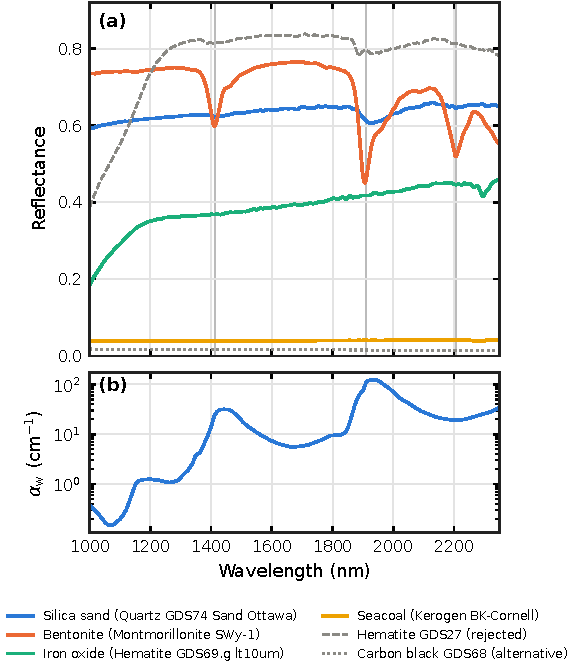
\includegraphics[width=\columnwidth]{figures/fig1_endmembers.pdf}
\caption{(a) Reference reflectance spectra in the 1000--2350\,nm window, with alternatives in gray. Vertical lines mark the bentonite bands near 1414, 1910 and 2206\,nm. (b) Absorption coefficient of liquid water~\cite{segelstein1981}; $\alpha_{\rm w}=\alphaFourteen$\,cm$^{-1}$ at 1450\,nm and \alphaNineteen\,cm$^{-1}$ at 1940\,nm.}\label{fig:endmembers}
\end{figure}

\subsection{Mixing model}

Compositions are expressed as mass percent of the dry mixture for bentonite, seacoal and iron oxide, with silica sand as the balance; moisture is mass percent of the wet mixture. Let $m_i$ be the dry mass fraction, $\rho_i$ the density, $d_i$ the effective grain diameter, and $R_i(\lambda)$ the reflectance of component $i$. We use Hapke's diffusive-reflectance relation~\cite{hapke2012}, appropriate for hemispherical (integrating-sphere) measurements:
\begin{equation}
R=\frac{1-\gamma}{1+\gamma},\qquad \gamma=\sqrt{1-w},
\end{equation}
which inverts in closed form as
\begin{equation}
w_i(\lambda)=1-\left(\frac{1-R_i(\lambda)}{1+R_i(\lambda)}\right)^{2}.
\end{equation}
Each component's share of geometric cross-section is
\begin{equation}
f_i=\frac{m_i/(\rho_i d_i)}{\sum_j m_j/(\rho_j d_j)},\label{eq:xs}
\end{equation}
and the mixture albedo and reflectance are
\begin{equation}
w_{\rm mix}(\lambda)=\sum_i f_i\,w_i(\lambda),\qquad R_{\rm mix}=\frac{1-\sqrt{1-w_{\rm mix}}}{1+\sqrt{1-w_{\rm mix}}}.\label{eq:mix}
\end{equation}
For comparison we also implement linear (areal) mixing, $R_{\rm mix}=\sum_i m_i R_i$, and absorbance-linear mixing, $A_{\rm mix}=\sum_i m_i A_i$ with $A=-\log_{10}R$. For the reference recipe of 8\% bentonite, 3\% seacoal and 0.5\% iron oxide, Eq.~\eqref{eq:xs} gives cross-section shares of \xsSand{} (sand), \xsClay{} (bentonite), \xsSc{} (seacoal) and \xsFe{} (iron oxide). The 3\% of seacoal thus covers about \xsSc{} of the grain cross-section. Appendix~\ref{app:worked} works through one library value by hand.

\subsection{Water film model}

Moisture is modeled as a uniform film on all grain surfaces. With moisture $\mu$ (mass percent of wet mixture), the water volume per gram of dry solids is $V_{\rm w}=\mu/[(100-\mu)\rho_{\rm w}]$, and the grain surface area per gram is $S=\sum_i 6m_i/(\rho_i d_i)$ for spheres. The film thickness is $t=V_{\rm w}/S$; for the reference recipe at 3.5\% moisture, $t=\filmThreeFive$\um. Each grain's albedo is attenuated by two passes through the film,
\begin{equation}
w_i'(\lambda)=w_i(\lambda)\exp\!\left[-2\kappa\,\alpha_{\rm w}(\lambda)\,t\right],\qquad \alpha_{\rm w}=\frac{4\pi k_{\rm w}}{\lambda},
\end{equation}
where $k_{\rm w}$ is the imaginary refractive index of water~\cite{segelstein1981} and $\kappa$ is a path-length factor. We set $\kappa=1$ (pure geometry), which ignores refractive-index darkening~\cite{lekner1988} and is therefore conservative; $\kappa=4$ is examined as a sensitivity case.

\subsection{Instrument model}

Spectra are resampled to the instrument class used in~\cite{kuubata2025}: an AvaSpec-NIR256-2.5TEC with a 256-pixel thermoelectrically cooled InGaAs array and an AvaSphere-50 integrating sphere, read over 1000--2350\,nm. Channel centers are spaced 6.93\,nm, matching the pixel spacing in the laboratory data, giving \nInst{} channels. Each channel has a Gaussian spectral response of 15\,nm full width at half maximum:
\begin{equation}
R_c=\frac{\sum_\lambda G_c(\lambda)R(\lambda)}{\sum_\lambda G_c(\lambda)},\quad G_c=\exp\!\left[-\frac{(\lambda-\lambda_c)^2}{2\sigma^2}\right].
\end{equation}
A simulated reading adds packing and instrument effects:
\begin{equation}
\tilde R_c=R_c(1+\epsilon_{\rm g})+\epsilon_{\rm o}+\epsilon_{\rm s}x_c+\epsilon_c,\label{eq:noise}
\end{equation}
where $\epsilon_{\rm g}$, $\epsilon_{\rm o}$ and $\epsilon_{\rm s}$ are per-spectrum random gain, offset and tilt (packing and presentation variation), $x_c$ is the channel position scaled to $[-\tfrac12,\tfrac12]$, and $\epsilon_c\sim\mathcal N\!\left(0,[\mathrm{SNR}\,\pi(\lambda_c)]^{-2}\right)$ is detector noise. The profile $\pi(\lambda)$ reduces the signal-to-noise ratio toward both edges of the extended InGaAs range (0.6 at 1000\,nm, 1.0 from 1100 to 2100\,nm, 0.3 at 2350\,nm). Three noise tiers are defined (Table~\ref{tab:noise}).

\begin{table}[t]
\caption{Noise tiers. SNR refers to a perfect white reflector at the best channels; the remaining columns are standard deviations of the terms in Eq.~\eqref{eq:noise}.}\label{tab:noise}
\centering\footnotesize
\begin{tabular}{@{}lcccc@{}}
\toprule
Tier & SNR & Gain sd & Offset sd & Tilt sd\\
\midrule
\tabinput{tables/tab_noise.tex}
\bottomrule
\end{tabular}
\end{table}

\subsection{Laboratory reference data}

The laboratory data are the 32 dry mixtures of~\cite{kuubata2025}: silica sand (AGSCO) with 3, 6, 9 and 12\% DC2 bentonite, each without additive and with 1, 3 and 5\% seacoal or 0.5, 1 and 2\% red iron oxide, blended for 10\,min, presented in a leveled petri dish against the sphere port, and measured in absorbance mode against a mirror reference (5\,ms integration, 100 scans averaged, detector at $-8\,^\circ$C). That study reports, for each additive series, PC1 scores from PCA on centered and scaled absorbance over 1000--2350\,nm, and a relative area under the curve,
\begin{equation}
\mathrm{AUC}_j=\int_{1000}^{2350}\left[A_j(\lambda)-A_{0,k(j)}(\lambda)\right]d\lambda,\label{eq:auc}
\end{equation}
evaluated by the trapezoid rule, where $A_{0,k}$ is the absorbance of the 0\% additive sample at the same DC2 level $k$. The 24 AUC and PC1 values for additive-containing samples were taken from the data tables of~\cite{kuubata2025} (Appendix~\ref{app:lab}) and verified by the author against the original spreadsheets. Because AUC is a difference within one instrument and session, it is insensitive to the reference standard, which makes it directly comparable with computed spectra.

\subsection{Calibration of effective particle sizes}

The effective sizes of silica sand (250\um, consistent with a sand of AFS grain fineness number 50--60) and bentonite (10\um, representing clay aggregates rather than individual platelets) are fixed by assumption. The effective sizes of seacoal and iron oxide are the least constrained inputs: both are fine powders that clump and coat sand grains during mulling. We calibrate them against the measured AUC values.

Within each DC2 group, all six AUC values (three seacoal, three iron oxide) are computed against the same single baseline spectrum. Any difference between that one baseline measurement and the additive samples, from packing, measurement session or reference drift, shifts all six values in the group by the same amount. We therefore fit one offset $b_k$ per DC2 group together with the two sizes:
\begin{equation}
\min_{d_{\rm sc},d_{\rm Fe},\{b_k\}}\sum_{j=1}^{24}\left[\mathrm{AUC}^{\rm lab}_j-\mathrm{AUC}^{\rm mod}_j(d_{\rm sc},d_{\rm Fe})-b_{k(j)}\right]^2.\label{eq:cal}
\end{equation}
For fixed sizes the optimal $b_k$ is the mean residual of group $k$, so the problem reduces to a two-dimensional search over a logarithmic grid of 45 sizes from 1 to 300\um{} each. Computed AUC values use the instrument model without noise. We evaluate every combination of seacoal and iron oxide stand-in spectra, and test stability by leaving out one DC2 group at a time. The offsets are reported as results, not hidden.

\subsection{Replication of the laboratory analysis}

To test whether the calibrated model reproduces the measured behavior, we recreate the laboratory design (16 spectra per additive series), apply lab-tier noise, and run exactly the laboratory analysis: PCA on centered, unit-variance absorbance columns (equivalent to R's \texttt{prcomp} with \texttt{scale.=TRUE}) and the relative AUC of Eq.~\eqref{eq:auc}. Five trends are checked over 50 independent noise realizations: (T1) PC1 explains more than 95\% of variance in both series; (T2, T3) PC1 scores rise with seacoal and with iron oxide (median Spearman $\rho>0.8$); (T4) AUC rises with additive level within every DC2 group in at least 95\% of realizations; (T5) the seacoal series reaches larger AUC than the iron oxide series. The same analysis is run with the assumed starting sizes and no laboratory calibration ($d_{\rm sc}=75$\um, $d_{\rm Fe}=5$\um) and with linear mixing.

\subsection{Library design}

The dry library v1.0 is a full factorial grid: bentonite 3--12\% in 1\% steps, seacoal 0--5\% in 0.25\% steps, and iron oxide 0--2\% in 0.1\% steps (\nDry{} recipes). The moisture extension crosses bentonite 3--12\% (1\% steps), seacoal 0--5\% (0.5\%), iron oxide 0--2\% (0.25\%), and moisture 2--5\% (0.5\%) (\nMoist{} recipes). Each recipe is stored as noise-free reflectance at 1\,nm (\nNative{} channels) and at instrument resolution (\nInst{} channels); noise is added at use time with Eq.~\eqref{eq:noise}. A quality-assurance report checks counts, physical ranges, and the direction of change with each absorber.

\subsection{Detection-limit benchmark}\label{sec:bench}

For each target additive (seacoal, iron oxide), each sand condition (dry; moist at 2--5\%), and each noise tier, we generate a calibration set and a test set (\nSets{} sets in total). Non-target components vary uniformly across production ranges (bentonite 3--12\%, the other additive across its full range, and moisture where applicable), so a method must detect the target against realistic background variation. Calibration sets hold \nCal{} spectra, 25\% with zero target and the rest log-uniformly distributed from the lowest test level to the maximum. Test sets hold \nTestBlank{} zero-level spectra and \nTestLevel{} spectra at each level: seacoal at \levelsSc\%, and iron oxide at \levelsFe\% (\nTestSc{} and \nTestFe{} test spectra).

A method trains on the calibration set and assigns each test spectrum a score $s$, higher meaning more target additive. The decision threshold $\tau$ is the 95th percentile of blank scores. Classifier probabilities often tie exactly at the threshold, so ties are resolved with the randomized Neyman--Pearson test~\cite{lehmann2005}: blank samples tied at $\tau$ are counted with the weight $q$ that makes the false-alarm rate exactly $\alpha$,
\begin{equation}
q=\frac{\alpha-P(s>\tau\mid0)}{P(s=\tau\mid0)},
\end{equation}
and the detection power at level $L$ is
\begin{equation}
\pi(L)=P(s>\tau\mid L)+q\,P(s=\tau\mid L).
\end{equation}
The detection limit is the lowest level at which power reaches 95\% and stays there at every higher level:
\begin{equation}
\mathrm{LOD}=\min\{L:\pi(L')\ge0.95\ \ \forall L'\ge L\}.\label{eq:lod}
\end{equation}
The requirement on higher levels matters for process control, where an alarm that fails at large deficits is unusable. We also report the lowest level reaching 95\% power, which reveals methods that detect low levels but miss high ones. The rule is fixed, published with the sets, and implemented in a scoring script that anyone can run on new methods.

\subsection{Baseline methods}

All baselines use absorbance $A=-\log_{10}\tilde R$ as input. We tested standard normal variate (SNV)~\cite{barnes1989}, multiplicative scatter correction~\cite{geladi1985} and Savitzky--Golay derivatives~\cite{savitzky1964,rinnan2009} for PLSR. Plain absorbance gave the lowest or equal error in nearly all conditions, because these corrections remove the broadband darkening that carries most of the seacoal signal. The baselines are:
\begin{itemize}\itemsep0pt
\item \textbf{PLSR}~\cite{wold2001}: regression on target percent; the number of latent variables (up to 20) is the smallest within 1\% of the minimum five-fold cross-validated RMSE (RMSECV); score $=$ predicted percent.
\item \textbf{PCA-LDA}: ten principal components followed by linear discriminant analysis of present versus absent, in the spirit of the PCA analysis of~\cite{kuubata2025}.
\item \textbf{SVM-RBF}~\cite{cortes1995}: support-vector classifier with radial basis kernel ($C=10$) on standardized absorbance.
\item \textbf{Random forest}~\cite{breiman2001}: 300 trees, present versus absent.
\item \textbf{Gradient boosting}~\cite{friedman2001}: histogram-based gradient-boosted trees, present versus absent.
\end{itemize}
Classifiers are trained to separate zero-target from target-containing calibration spectra and score with their decision function or class probability.

\subsection{Sensitivity analysis and software}

The PLSR detection limit (dry sand, lab tier) is recomputed under alternative assumptions: assumed starting sizes without laboratory calibration, linear mixing, carbon black as seacoal, calcium montmorillonite SAz-1 as bentonite, a 30\um{} bentonite size, and a 25\,nm instrument response; for moist sand, a water path factor $\kappa=4$. The pipeline is implemented in Python with NumPy~\cite{harris2020}, SciPy~\cite{virtanen2020}, scikit-learn~\cite{pedregosa2011} and Matplotlib~\cite{hunter2007}. It runs end to end in a few minutes with fixed random seeds, and reproduces identical outputs when rerun from an empty directory.

\section{Results}\label{sec:results}

\subsection{Validation of the mixing model}

As an independent check, we compare the mixing rules on a measured USGS mixture of 2\% hematite and 98\% fine quartz (GDS76). Hapke mixing reproduces the measured spectrum with RMSE \mmRmseHapke{} over 1000--2350\,nm, against \mmRmseLinear{} for linear mixing (Fig.~\ref{fig:gds76}). The difference is concentrated at the iron oxide edge: at 1000\,nm the measured reflectance is \mmRthousandMeasured, Hapke mixing gives \mmRthousandHapke{} and linear mixing \mmRthousandLinear. Relative to the quartz end-member, 2\% of hematite lowers the 1000\,nm reflectance by \dropMeas, about \dropRatio{} times the \dropLin{} that linear mixing predicts; Hapke mixing predicts \dropHapke, as the cross-section weighting implies.

\begin{figure}[t]
\centering
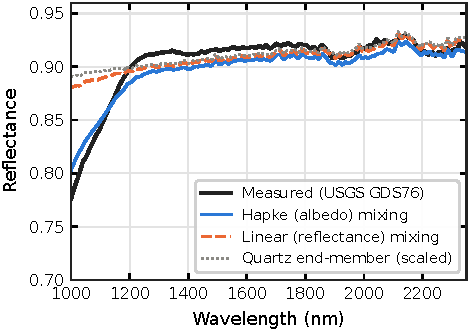
\includegraphics[width=\columnwidth]{figures/fig2_gds76.pdf}
\caption{Mixing-model check on the measured USGS 2\% hematite + 98\% quartz mixture (GDS76). The quartz end-member is scaled to the mixture's long-wavelength level (factor \mmQuartzScale) because the GDS76 quartz is brighter than GDS31.}\label{fig:gds76}
\end{figure}

\subsection{Calibration against laboratory mixtures}\label{sec:calres}

Table~\ref{tab:candidates} compares all stand-in combinations. The bright synthetic hematite GDS27 cannot reproduce the measured AUC increase at any particle size: its reflectance exceeds that of the sand from about 1135\,nm onward (Fig.~\ref{fig:endmembers}a), so adding it lowers absorbance on average and the computed AUC is never positive. Both darker hematites fit the data, as do both seacoal stand-ins, with RMSE near \rmseOff. We adopt kerogen and hematite GDS69 ($<$10\um) as defaults.

\begin{table}[t]
\caption{Calibration against the 24 measured AUC values for each combination of stand-in spectra: fitted effective sizes, RMSE with per-group offsets, and the maximum computed iron oxide AUC.}\label{tab:candidates}
\centering\footnotesize
\setlength{\tabcolsep}{2.5pt}
\begin{tabular}{@{}llcccc@{}}
\toprule
Seacoal & Iron oxide & $d_{\rm sc}$ ($\mu$m) & $d_{\rm Fe}$ ($\mu$m) & RMSE & max AUC$_{\rm Fe}$\\
\midrule
\tabinput{tables/tab_candidates.tex}
\bottomrule
\multicolumn{6}{@{}p{\columnwidth}@{}}{\scriptsize $^\ddagger$Upper bound of the search grid; no positive AUC at any size.}
\end{tabular}
\end{table}

The fitted sizes are $d_{\rm sc}=\dSc$\um{} and $d_{\rm Fe}=\dFe$\um{} (Fig.~\ref{fig:calib}a). Leaving out one DC2 group at a time moves them within \dScLo--\dScHi\um{} and \dFeLo--\dFeHi\um{} (Table~\ref{tab:loo}). The seacoal value is about half the 75\um{} prior used for the uncalibrated model, consistent with fines and grain coating produced during mixing. The iron oxide value lies below the wavelength, where Hapke theory is only approximate, so we treat it as an empirical parameter.

\begin{table}[t]
\caption{Leave-one-DC2-group-out stability of the calibration.}\label{tab:loo}
\centering\footnotesize
\begin{tabular}{@{}cccc@{}}
\toprule
Left-out DC2 (\%) & $d_{\rm sc}$ ($\mu$m) & $d_{\rm Fe}$ ($\mu$m) & RMSE (A$\cdot$nm)\\
\midrule
\tabinput{tables/tab_loo.tex}
\bottomrule
\end{tabular}
\end{table}

\begin{figure*}[t]
\centering
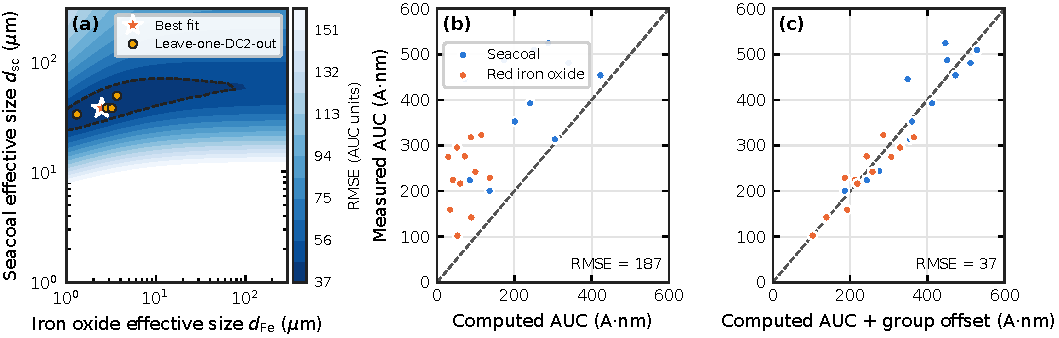
\includegraphics[width=\textwidth]{figures/fig3_calibration.pdf}
\caption{Calibration against the measured relative AUC of~\cite{kuubata2025}. (a) RMSE of Eq.~\eqref{eq:cal} over the two effective sizes; the dashed contour encloses RMSE within 25\% of the minimum. (b) Computed AUC alone versus measured. (c) Computed AUC plus one shared offset per DC2 group versus measured.}\label{fig:calib}
\end{figure*}

The offsets are large: \offThree, \offSix, \offNine{} and \offTwelve{} absorbance$\cdot$nm for the 3, 6, 9 and 12\% DC2 groups, equivalent to mean absorbance shifts of \offAbsLo--\offAbsHi{} across the 1350\,nm window. Without them, computed and measured AUC differ by \rmseRaw{} units RMSE (Fig.~\ref{fig:calib}b); with them, by \rmseOff{} (Fig.~\ref{fig:calib}c; correlation \rFitSc{} for seacoal and \rFitFe{} for iron oxide; largest residual \residMaxAbs). Offsets alone, with no additive model, leave an RMSE of \rmseOffOnly, close to the standard deviation of the measurements (\labAucSd), so the composition model carries the within-group structure. Appendix~\ref{app:lab} lists every measured and computed value.

\subsection{Replication of laboratory trends}

Table~\ref{tab:trends} summarizes the replication. The calibrated model reproduces all five trends: PC1 explains \pcScCal\% of variance for seacoal (measured 99.23\%) and \pcFeCal\% for iron oxide (measured 97.87\%), PC1 rises with both additives, and AUC rises with every additive step in every DC2 group. The assumed starting sizes without calibration reproduce \trendsUsgs{} trends and linear mixing \trendsLin.

\begin{table*}[t]
\caption{Replication of the laboratory analysis on computed spectra (lab-tier noise, 50 realizations). PC1: median variance explained (\%); $\rho$: median Spearman correlation of PC1 with additive level; Mono.: share of realizations with AUC rising at every step; RMSE: computed versus measured AUC with group offsets (A$\cdot$nm). Measured values: PC1 99.23\% (seacoal) and 97.87\% (iron oxide).}\label{tab:trends}
\centering\footnotesize
\begin{tabular}{@{}lccccccccccc@{}}
\toprule
Model & PC1$_{\rm sc}$ & PC1$_{\rm Fe}$ & $\rho_{\rm sc}$ & $\rho_{\rm Fe}$ & Mono. & RMSE & T1 & T2 & T3 & T4 & T5\\
\midrule
\tabinput{tables/tab_trends.tex}
\bottomrule
\end{tabular}
\end{table*}

Figure~\ref{fig:pc1} compares PC1 scores directly. Computed and measured scores share the same range and the same rise with additive content. The differences are instructive. Measured scores jump at the first additive step (from between $-25$ and $-14$ at 0\% seacoal to between $-9$ and $+11$ at 1\%) and then rise more slowly. They also order by DC2 opposite to the computed scores: higher DC2 gives higher measured scores but lower computed ones. Both features are what a shared baseline offset produces. In the model, more bentonite dilutes the additive's share of cross-section, so the additive effect per percent falls slightly with clay content.

\begin{figure*}[t]
\centering
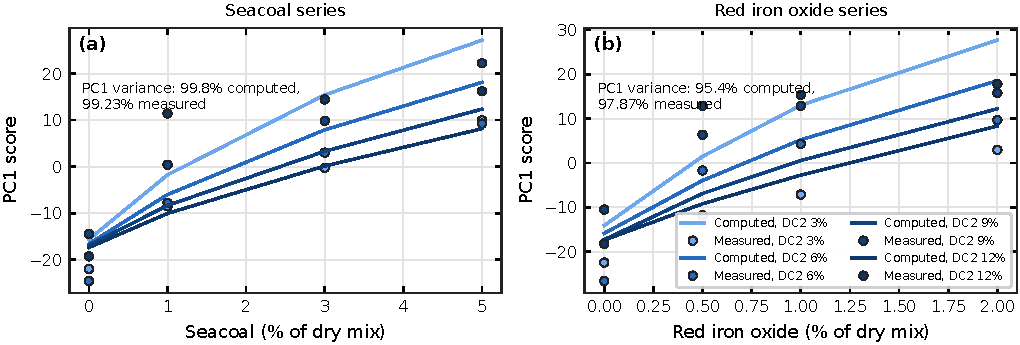
\includegraphics[width=\textwidth]{figures/fig4_pc1.pdf}
\caption{PC1 scores versus additive level for the laboratory design: measured values of~\cite{kuubata2025} (markers) and computed values with the calibrated model (lines, mean of 50 noise realizations), colored by DC2 level. (a) Seacoal series. (b) Red iron oxide series.}\label{fig:pc1}
\end{figure*}

\subsection{The library}

The QA report confirms \nDry{} dry and \nMoist{} moist spectra, all finite and within $(0,1)$. More seacoal lowers mean reflectance in every one of the 4200 neighboring grid steps, more iron oxide lowers 1000--1020\,nm reflectance in every step, and more moisture lowers mean reflectance in every step. Over the full window, more iron oxide lowers mean reflectance in \feFullShare\% of steps. The exceptions are the darkest high-seacoal recipes, which are already darker than the hematite itself, so added hematite lightens the average. Figure~\ref{fig:library} shows representative series. Seacoal darkens the spectrum broadly and nonlinearly, with the first percent producing the largest change. Iron oxide darkens most strongly at the short-wavelength edge. Bentonite deepens the 1410, 1910 and 2205\,nm bands while brightening the continuum, because SWy-1 is brighter than the sand outside its bands.

\begin{figure*}[t]
\centering
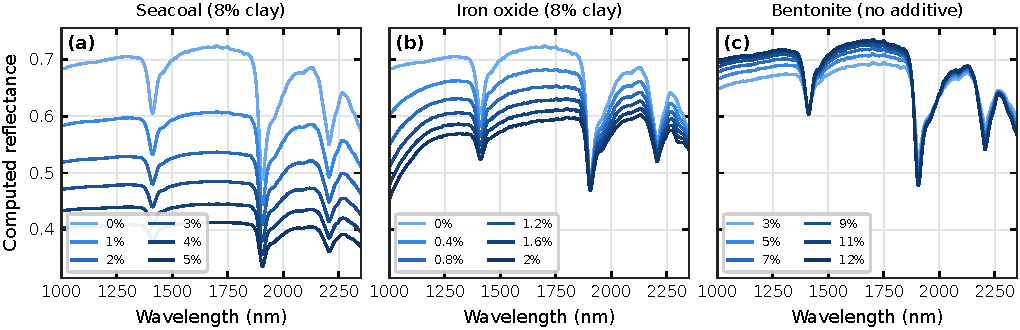
\includegraphics[width=\textwidth]{figures/fig5_library.pdf}
\caption{Library v1.0 examples (noise-free, 1\,nm). (a) Seacoal 0--5\% at 8\% bentonite. (b) Iron oxide 0--2\% at 8\% bentonite. (c) Bentonite 3--12\% without additives. Darker lines carry more of the varied component.}\label{fig:library}
\end{figure*}

\subsection{Moisture extension}

Water adds absorption at 1450 and 1940\,nm and slight broadband darkening (Fig.~\ref{fig:moist}). For the reference recipe, reflectance at 1940\,nm falls from \RnineteenDry{} (dry) to \RnineteenWetTwo{} at 2\% moisture and \RnineteenWetFive{} at 5\%. These changes are modest because the film is thin (\filmThreeFive\um{} at 3.5\%) and $\kappa=1$. Real moist green sand is likely darker (Sec.~\ref{sec:limits}).

\begin{figure}[t]
\centering
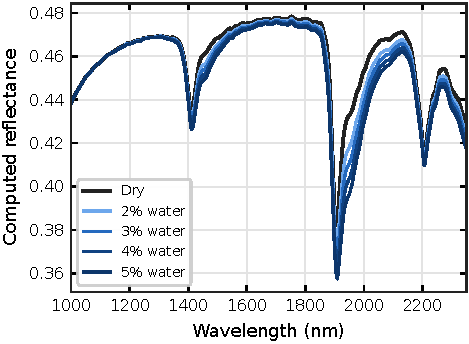
\includegraphics[width=\columnwidth]{figures/fig6_moisture.pdf}
\caption{Moisture extension: reference recipe (8\% bentonite, 3\% seacoal, 0.5\% iron oxide) dry and at 2--5\% moisture.}\label{fig:moist}
\end{figure}

\subsection{Detection limits}

Figure~\ref{fig:power} shows detection power versus level for dry sand at lab-tier noise, and Table~\ref{tab:lod} and Fig.~\ref{fig:heat} give detection limits for all methods and conditions. PLSR is the most consistent method. It detects seacoal from \lodScDryLab\% and iron oxide from \lodFeDryLab\% at lab-tier noise, from \lodScDryIdeal\% and \lodFeDryIdeal\% at ideal noise, and from \lodScDryPlant\% and \lodFeDryPlant\% at plant-floor noise. In moist sand the limits are \lodScMoistLab\% and \lodFeMoistLab\% (lab tier) and \lodScMoistPlant\% and \lodFeMoistPlant\% (plant tier). At its limit, PLSR flags iron oxide at concentrations about one fifth of those for seacoal: iron oxide acts through a spectral edge as well as through broadband darkening, while seacoal's broadband effect is partly mimicked by packing variation and by the darkening from other components. Below the limits, power falls smoothly; for example, PLSR detects 0.3\% seacoal in \powScThree{} of samples and 0.05\% iron oxide in \powFeFive.

\begin{figure*}[t]
\centering
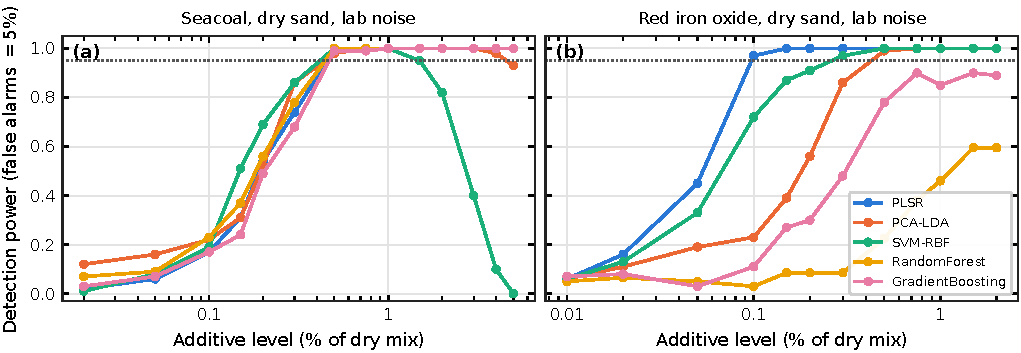
\includegraphics[width=\textwidth]{figures/fig7_power.pdf}
\caption{Detection power (share of test samples above the threshold, with false alarms held at 5\%) versus additive level, dry sand, lab-tier noise. The dotted line marks 95\%. (a) Seacoal. (b) Red iron oxide.}\label{fig:power}
\end{figure*}

\begin{table*}[t]
\caption{Detection limits (\% of dry mix) for every baseline and condition, Eq.~\eqref{eq:lod}. Bold: best in column. n.r.: not reached at any level; $^\dagger$: 95\% power reached at some level but lost at a higher level.}\label{tab:lod}
\centering\footnotesize
\setlength{\tabcolsep}{4pt}
\begin{tabular}{@{}lcccccccccccc@{}}
\toprule
 & \multicolumn{6}{c}{Seacoal} & \multicolumn{6}{c}{Red iron oxide}\\
\cmidrule(lr){2-7}\cmidrule(l){8-13}
 & \multicolumn{3}{c}{Dry} & \multicolumn{3}{c}{Moist} & \multicolumn{3}{c}{Dry} & \multicolumn{3}{c}{Moist}\\
\cmidrule(lr){2-4}\cmidrule(lr){5-7}\cmidrule(lr){8-10}\cmidrule(l){11-13}
Method & Ideal & Lab & Plant & Ideal & Lab & Plant & Ideal & Lab & Plant & Ideal & Lab & Plant\\
\midrule
\tabinput{tables/tab_lod.tex}
\bottomrule
\end{tabular}
\end{table*}

\begin{figure*}[t]
\centering
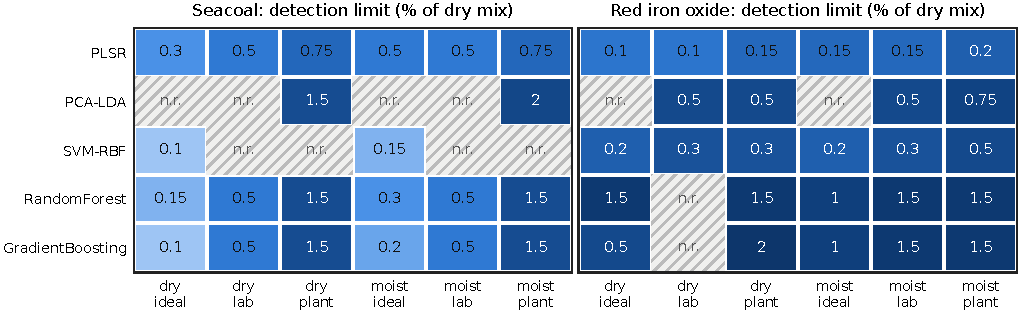
\includegraphics[width=\textwidth]{figures/fig8_lod_heatmap.pdf}
\caption{Detection limits by method and condition (darker = higher limit). Hatched cells: not reached under Eq.~\eqref{eq:lod}.}\label{fig:heat}
\end{figure*}

The classifiers behave differently. At ideal noise, SVM and gradient boosting reach lower seacoal limits than PLSR (0.1\%), because they capture the nonlinear saturation of the seacoal response that a linear model cannot. Under realistic noise, several classifiers fail the requirement on higher levels. The SVM detects every seacoal sample at 1\% (power \svmOne) but none at 5\% (power \svmFive), and PCA-LDA loses power at 5\%. A classifier trained to separate ``present'' from ``absent'' has no reason to keep its decision function increasing beyond the region where the classes are hardest to separate, so it can miss gross deficits. Tree ensembles detect iron oxide poorly at lab-tier noise (random forest power \rfFeTwo{} at 2\%), consistent with the weak, distributed edge signal being hard to capture with axis-aligned splits on noisy channels. Table~\ref{tab:plsr} gives PLSR diagnostics; Fig.~\ref{fig:pred} shows the curvature of PLSR predictions for seacoal, which a nonlinear regression could exploit.

\begin{table}[t]
\caption{PLSR diagnostics: latent variables (LV), cross-validated RMSE (\% of dry mix), cross-validated $R^2$, and detection limit.}\label{tab:plsr}
\centering\footnotesize
\setlength{\tabcolsep}{3pt}
\begin{tabular}{@{}lllcccc@{}}
\toprule
Target & Sand & Noise & LV & RMSECV & $R^2_{\rm CV}$ & LOD\\
\midrule
\tabinput{tables/tab_plsr.tex}
\bottomrule
\end{tabular}
\end{table}

\begin{figure*}[t]
\centering
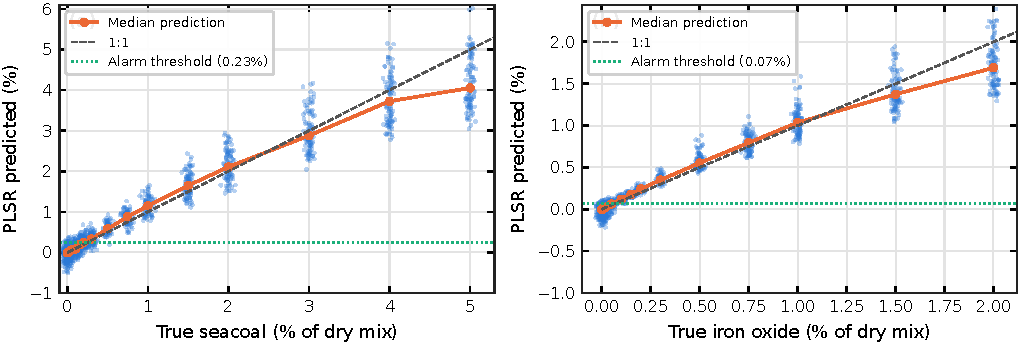
\includegraphics[width=\textwidth]{figures/fig9_plsr_pred.pdf}
\caption{PLSR predictions on the dry, lab-tier test sets (points jittered horizontally). The dotted line is the decision threshold that holds false alarms at 5\%. (a) Seacoal: threshold \thrSc\%, prediction RMSE \rmsepSc\%. (b) Red iron oxide: threshold \thrFe\%, RMSE \rmsepFe\%.}\label{fig:pred}
\end{figure*}

\subsection{Sensitivity to modeling assumptions}

Table~\ref{tab:sens} and Fig.~\ref{fig:sens} show how the PLSR limits respond to each assumption. Most alternatives move the limits by at most one grid level. Carbon black as seacoal and calcium montmorillonite as bentonite lower the seacoal limit to \sensScCb\% and \sensScSaz\%, uncalibrated priors give \sensScUsgs\% and \sensFeUsgs\%, and a 25\,nm instrument response leaves the limits at \sensScFwhm\% and \sensFeFwhm\%. The exception is linear mixing, which raises the limits to \sensScLin\% and \sensFeLin\%: the choice of mixing physics, not the choice of stand-in spectra, is the decisive assumption. For moist sand, raising the water path factor to $\kappa=4$ gives \moistScPf\% and \moistFePf\% (\moistScDef\% and \moistFeDef\% at $\kappa=1$).

\begin{table}[t]
\caption{Sensitivity of the PLSR detection limit (dry sand, lab tier; \%) and RMSECV to modeling assumptions.}\label{tab:sens}
\centering\footnotesize
\setlength{\tabcolsep}{2.5pt}
\begin{tabular}{@{}p{3.0cm}cccc@{}}
\toprule
 & \multicolumn{2}{c}{Seacoal} & \multicolumn{2}{c}{Iron oxide}\\
\cmidrule(lr){2-3}\cmidrule(l){4-5}
Scenario & LOD & RMSECV & LOD & RMSECV\\
\midrule
\tabinput{tables/tab_sens.tex}
\bottomrule
\end{tabular}
\end{table}

\begin{figure}[t]
\centering
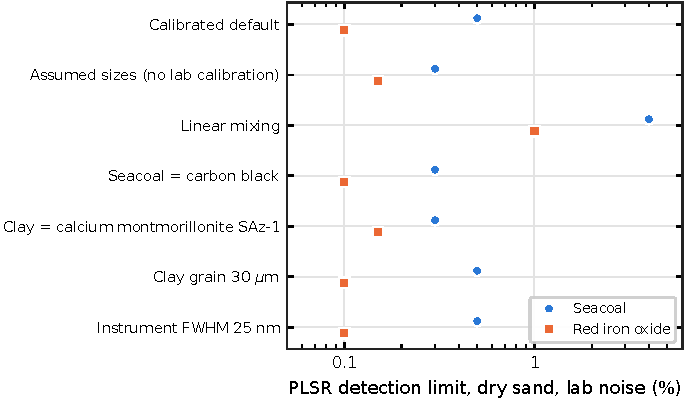
\includegraphics[width=\columnwidth]{figures/fig10_sensitivity.pdf}
\caption{PLSR detection limits under alternative assumptions (dry sand, lab tier).}\label{fig:sens}
\end{figure}

\section{Discussion}\label{sec:discussion}

\subsection{What the detection limits mean for a foundry}

Under the stated assumptions, a PLSR calibration on an InGaAs instrument of this class can, in principle, flag a seacoal change of about half a percent of the dry mix and an iron oxide change of about a tenth of a percent, with one false alarm in twenty clean samples, while clay, the other additive, and moisture vary across production ranges. At plant-floor noise these figures rise to about three quarters of a percent and 0.15--0.2\%. These are limits for detecting presence against zero. Tracking a change around a nonzero operating point is easier, because the response is steepest near zero for seacoal (Fig.~\ref{fig:library}a) and the background is narrower in a single plant. The numbers therefore bound what an NIR sensor could add to LOI-based control: a reading in seconds that resolves seacoal to roughly the half-percent level within the 0--5\% range studied, instead of a laboratory result that arrives after the sand is in molds.

The benchmark also shows that method choice matters as much as instrument noise. A classifier with an excellent low-level detection rate can still miss the largest deficits, which is precisely the failure a process alarm cannot tolerate. Requiring detection at every higher level, as Eq.~\eqref{eq:lod} does, exposes this. We recommend that NIR calibrations for sand control report power curves, not only cross-validated error.

\subsection{Lessons for laboratory design}

The shared-baseline component in the laboratory AUC values has a practical implication for future measurements. When every additive sample in a group is referenced to a single baseline sample, any error in that one measurement enters every derived value in the group and can masquerade as a clay effect. The two-way ANOVA in~\cite{kuubata2025} found a DC2 effect on AUC (significant at $p<0.01$ for the red iron oxide series); the present analysis suggests that part of that effect may come from the baselines. Replicated baselines measured in the same session as the additive samples, and randomized run order across groups, would separate the two. The calibration here is robust to the offsets by construction, but it cannot recover the true clay dependence of the additive effect, which in the model decreases slightly with clay content.

\subsection{Limitations}\label{sec:limits}

The library is computed, not measured. It inherits the limitations of its inputs and of the mixing model. (i) The USGS library contains no coal and no foundry-grade red iron oxide; kerogen and natural hematite are stand-ins. The seacoal limit is insensitive to the stand-in (Table~\ref{tab:sens}), but measured spectra of the actual materials are the most valuable improvement. (ii) The effective sizes of seacoal and iron oxide are fitted to 24 dry values from one study with one sand and one bentonite. The iron oxide size lies below the wavelength, where the theory is approximate. (iii) The source study describes DC2 as a southern (calcium) bentonite in its methods and as a western (sodium) bentonite in figure legends. The library uses sodium montmorillonite; calcium montmorillonite changes the seacoal limit by one level. (iv) The water model is a geometric film with $\kappa=1$. It omits refractive-index darkening~\cite{lekner1988}, interlayer water, and compaction, and has not been calibrated against measured moist green sand; the moisture extension is a first approximation. (v) Noise tiers are stated levels, not estimates from replicate scans of a specific instrument, and the 15\,nm response width is assumed. (vi) The laboratory measurements used a mirror reference, whereas the library is relative to a perfect diffuse reflector. Differences of this kind cancel in relative AUC and in calibrations built within one instrument, but absolute absorbances are not comparable. (vii) The library omits burnt (dead) clay, oolitic coatings, fines, other carbon carriers, temperature and system aging. (viii) Benchmark test labels are public, so the leaderboard relies on good faith, with methods expected to publish code.

\subsection{Future work}

The natural next steps are: measured spectra of the actual materials (AGSCO sand, DC2 bentonite, foundry seacoal and red iron oxide) on the same instrument; replicate scans to set the lab noise tier from data; measured moist and compacted green sand at 2--5\% water to calibrate $\kappa$ and add a compaction term; additional carbon carriers and dead clay; and external validation against plant samples with LOI and methylene blue results. Each can be added as a new library version without changing the benchmark rule, so results remain comparable across versions.

\section{Conclusions}\label{sec:conclusions}

We have built and released an open NIR reference for green sand additive control: \nTotal{} computed spectra across production ranges of bentonite, seacoal, red iron oxide and moisture; a calibration of the mixing model against measured laboratory mixtures that reproduces all five laboratory trends tested; a detection-limit benchmark with a fixed two-error scoring rule; and a tested Python package. With laboratory-grade noise, PLSR detects seacoal from \lodScDryLab\% and red iron oxide from \lodFeDryLab\% of the dry mix, and from \lodScDryPlant\% and \lodFeDryPlant\% at plant-floor noise. Some machine-learning classifiers detect low levels but miss high ones, a failure the benchmark is designed to expose. Linear mixing would overstate the detection limits several-fold, so particulate radiative transfer is essential to any computed reference of this kind. The analysis also identifies a shared-baseline component in the laboratory data, with a concrete recommendation for future measurement design. Any foundry, sensor maker or researcher can now test a calibration against the same open reference and report a detection limit that others can check.

\section*{Data and code availability}

All data, code, documentation and the leaderboard are available at \url{https://github.com/mauricekuubata/greensand-nir}~\cite{greensandnir} and are archived on Zenodo as four versioned records (library v1.0, benchmark, moisture extension, and software), whose DOIs are listed in the repository. Data are released under CC BY 4.0 and code under the MIT License. USGS spectra are in the U.S. public domain; the water optical constants are CC0.

\section*{Author contributions and use of AI tools}

M.K.: conceptualization, methodology, laboratory investigation (the source study), validation, data curation, and writing. M.K.\ set every mixing rule and verified every output. Claude (Anthropic), an AI assistant, assisted with code, data handling and drafting under the author's direction. The author takes full responsibility for the content.

\section*{Acknowledgments}

The author thanks the University of Northern Iowa Metal Casting Center, where the laboratory measurements were made, and the U.S. Geological Survey Spectroscopy Laboratory for the public spectral library.

\section*{Competing interests}

The author declares no competing interests. This work received no specific funding.

\appendix
\section{Measured and computed relative AUC}\label{app:lab}

Table~\ref{tab:labdata} lists the 24 measured relative AUC values of~\cite{kuubata2025} with the computed values from the calibrated model, the fitted DC2-group offsets, and the residuals.

\begin{table*}[t]
\caption{Measured AUC~\cite{kuubata2025}, computed AUC, group offset, and residual (absorbance$\cdot$nm). RIO: red iron oxide.}\label{tab:labdata}
\centering\footnotesize
\setlength{\tabcolsep}{6pt}
\begin{tabular}{@{}lccccccc@{}}
\toprule
Sample & Additive & DC2 & \% & Meas. & Comp. & Offset & Resid.\\
\midrule
\tabinput{tables/tab_labdata.tex}
\bottomrule
\end{tabular}
\end{table*}

\section{Worked example of the mixing rule}\label{app:worked}

Table~\ref{tab:worked} computes library recipe \texttt{\spotId} (88.5\% sand, 8\% bentonite, 3\% seacoal, 0.5\% iron oxide) at 1700\,nm. The mixture albedo is $w_{\rm mix}=\wMix$, giving $R=\RMix$, identical to the stored library value (\spotR). The calculation can be repeated in a spreadsheet.

\begin{table}[h]
\caption{Worked example at 1700\,nm. $a=m/(\rho d)$ in units of $10^{-3}$\,cm$^3$\,g$^{-1}\mu$m$^{-1}$; $f$: cross-section share.}\label{tab:worked}
\centering\scriptsize
\setlength{\tabcolsep}{2.4pt}
\begin{tabular}{@{}lccccccc@{}}
\toprule
 & $m$ & $\rho$ & $d$ & $R$ & $w$ & $a$ & $f$\\
\midrule
\tabinput{tables/tab_worked.tex}
\bottomrule
\end{tabular}
\end{table}

\small
\bibliographystyle{unsrtnat}
\bibliography{refs}

\end{document}
